\documentclass[12pt,letterpaper]{article}
\usepackage{graphicx,textcomp}
\usepackage{natbib}
\usepackage{setspace}
\usepackage{fullpage}
\usepackage{color}
\usepackage[reqno]{amsmath}
\usepackage{amsthm}
\usepackage{fancyvrb}
\usepackage{amssymb,enumerate}
\usepackage[T1]{fontenc}
\usepackage[all]{xy}
\usepackage{endnotes}
\usepackage{lscape}
\newtheorem{com}{Comment}
\usepackage{float}
\usepackage{hyperref}
\newtheorem{lem} {Lemma}
\newtheorem{prop}{Proposition}
\newtheorem{thm}{Theorem}
\newtheorem{defn}{Definition}
\newtheorem{cor}{Corollary}
\newtheorem{obs}{Observation}
\usepackage[compact]{titlesec}
\usepackage{dcolumn}
\usepackage{tikz}
\usetikzlibrary{arrows}
\usepackage{multirow}
\usepackage{xcolor}
\newcolumntype{.}{D{.}{.}{-1}}
\newcolumntype{d}[1]{D{.}{.}{#1}}
\definecolor{light-gray}{gray}{0.65}
\usepackage{url}
\usepackage{listings}
\usepackage{color}

\definecolor{codegreen}{rgb}{0,0.6,0}
\definecolor{codegray}{rgb}{0.5,0.5,0.5}
\definecolor{codepurple}{rgb}{0.58,0,0.82}
\definecolor{backcolour}{rgb}{0.95,0.95,0.92}

\lstdefinestyle{mystyle}{
	backgroundcolor=\color{backcolour},   
	commentstyle=\color{codegreen},
	keywordstyle=\color{magenta},
	numberstyle=\tiny\color{codegray},
	stringstyle=\color{codepurple},
	basicstyle=\footnotesize,
	breakatwhitespace=false,         
	breaklines=true,                 
	captionpos=b,                    
	keepspaces=true,                 
	numbers=left,                    
	numbersep=5pt,                  
	showspaces=false,                
	showstringspaces=false,
	showtabs=false,                  
	tabsize=2
}
\lstset{style=mystyle}
\newcommand{\Sref}[1]{Section~\ref{#1}}
\newtheorem{hyp}{Hypothesis}

\title{Problem Set 1}
\date{Due: October 8, 2026}
\author{Applied Stats/Quant Methods 1}

\begin{document}
	\maketitle
	
	\section*{Instructions}
	\begin{itemize}
	\item Please show your work! You may lose points by simply writing in the answer. If the problem requires you to execute commands in \texttt{R}, please include the code you used to get your answers. Please also include the \texttt{.R} file that contains your code. If you are not sure if work needs to be shown for a particular problem, please ask.
\item Your homework should be submitted electronically on GitHub.
\item This problem set is due before 23:59 on Thursday October 8, 2026. No late assignments will be accepted.
	\end{itemize}
	
	\vspace{1cm}
	\section*{Question 1: Education}

A school counselor was curious about the average of IQ of the students in her school and took a random sample of 25 students' IQ scores. The following is the data set:\\
\vspace{.5cm}

\lstinputlisting[language=R, firstline=37, lastline=37]{PS01_answers_codefile_NF.R}  

\vspace{1cm}

\begin{enumerate}
	\item Find a 90\% confidence interval for the average student IQ in the school (As a hint, you first need the mean and SD to create a CI

\vspace{4cm}

Let's start by doing it manually.
I have "n" show me how many students are in the sample.
\lstinputlisting[language=R, firstline=47, lastline=48]{PS01_answers_codefile_NF.R} 
Result: 
\begin{verbatim}
	> n
	[1] 25
\end{verbatim}
Because n=25 is less than 30, we will need to conduct a t-test rather than a z-test.

Then I calculate the mean of the sample.
\lstinputlisting[language=R, firstline=51, lastline=52]{PS01_answers_codefile_NF.R}  
Result:
\begin{verbatim}
	> y_mean
	[1] 98.44
\end{verbatim}

I calculate the standard deviation of the sample.
\lstinputlisting[language=R, firstline=55, lastline=56]{PS01_answers_codefile_NF.R}  
Result:
\begin{verbatim}
	> sd_y
	[1] 13.09287
\end{verbatim}

I calculate the standard error of the sample.
\lstinputlisting[language=R, firstline=60, lastline=61]{PS01_answers_codefile_NF.R}  
Result:
\begin{verbatim}
	> std_error
	[1] 2.618575
\end{verbatim}

Once that is done, I can calculate my t-statistic:
\indent The "alpha" is 0.1 because the confidence interval we are looking for is 90.   \\
\lstinputlisting[language=R, firstline=64, lastline=64]{PS01_answers_codefile_NF.R}  
\vspace{.25cm}
\indent The degrees of freedom are n-1:
\lstinputlisting[language=R, firstline=65, lastline=65]{PS01_answers_codefile_NF.R}
\begin{verbatim}
	> degrees_of_freedom
	[1] 24
\end{verbatim} 
That allows us to calculate the t critical value:
 \lstinputlisting[language=R, firstline=67, lastline=68]{PS01_answers_codefile_NF.R}
 Result:
 \begin{verbatim}
 	> t_score
 	[1] 1.710882
 \end{verbatim} 
 
 I then calculate the margins of error:
 \lstinputlisting[language=R, firstline=79, lastline=80]{PS01_answers_codefile_NF.R}
 Result:
 \begin{verbatim}
 	> margin_error
 	[1] 4.480072
 \end{verbatim} 
 
 With the margins of error, I can determine the upper and lower bounds of the confidence interval:
 \lstinputlisting[language=R, firstline=82, lastline=85]{PS01_answers_codefile_NF.R}
 Result:
 \begin{verbatim}
 	> print(c(lower_bound, upper_bound))
 	[1]  93.95993 102.92007
 \end{verbatim} 
 
 Now we can check our result with the R-commands:
  \lstinputlisting[language=R, firstline=90, lastline=94]{PS01_answers_codefile_NF.R} 
 Result: 
 \begin{verbatim}
 	> print(confidence_interval)
 	[1]  93.95993 102.92007
 	attr(,"conf.level")
 	[1] 0.9
 \end{verbatim}
 We find the same! We can conclude: \\

\textbf{A 90\% confidence interval for the average student IQ in the school would be between 93.96 and 102.92 (rounded). That means that if we sample a hundred times, 90\% of the time we will be right and the average will lie in that interval.}

\vspace{1cm}

	
	\item Next, the school counselor was curious  whether  the average student IQ in her school is higher than the average IQ score (100) among all the schools in the country.\\ 
	
	\noindent Using the same sample, conduct the appropriate hypothesis test with $\alpha=0.05$.
\end{enumerate}

As a reminder, we have: \\
n = 25 \\
mean of y = 98.44 \\
mean among all schools of the country = 100 \\
\lstinputlisting[language=R, firstline=107, lastline=107]{PS01_answers_codefile_NF.R} 

We can guess that the mean of the school is lower than the country-wide mean, but is the difference between both statistically different?
We are therefore conducting a one-sided test to check if the average student IQ of the counselor's school is actually higher than the average score among all schools.

We formulate these hypotheses: \\
H0: y{\_mean} $\leq$ y{\_mean\_country}  \\
H1: y{\_mean} >  y{\_mean\_country} \\
\vspace{.25cm}

We then calculate the t-statistic: 
 \lstinputlisting[language=R, firstline=118, lastline=119]{PS01_answers_codefile_NF.R} 
Result: 
\begin{verbatim}
	> t_statistic
	[1] -0.5957439
\end{verbatim}
\vspace{1cm}

We then need to calculate the corresponding p-value, with help of the degrees of freedom:
\lstinputlisting[language=R, firstline=121, lastline=121]{PS01_answers_codefile_NF.R} 
Result: 
\begin{verbatim}
	> df
	[1] 24
\end{verbatim}

p-value:
\lstinputlisting[language=R, firstline=125, lastline=126]{PS01_answers_codefile_NF.R} 
Result: 
\begin{verbatim}
	pt(t_statistic, df, lower.tail = FALSE)
	[1] 0.7215383
\end{verbatim}

\textbf {We can now draw a conclusion: because the p-value is above the threshold of 0,05, we fail to reject the null hypothesis according to which the school's average IQ is equal or inferior to the average IQ in the country. This is coherent with our original guess.}







\newpage

	\section*{Question 2: Political Economy}

\noindent Researchers are curious about what affects the amount of money communities spend on addressing homelessness. The following variables constitute our data set about social welfare expenditures in the USA. \\
\vspace{.5cm}


\begin{tabular}{r|l}
	\texttt{State} &\emph{50 states in US} \\
	\texttt{Y} & \emph{per capita expenditure on shelters/housing assistance in state}\\
	\texttt{X1} &\emph{per capita personal income in state} \\
	\texttt{X2} &  \emph{Number of residents per 100,000 that are "financially insecure" in state}\\
	\texttt{X3} &  \emph{Number of people per thousand residing in urban areas in state} \\
	\texttt{Region} &  \emph{1=Northeast, 2= North Central, 3= South, 4=West} \\
\end{tabular}

\vspace{.5cm}
\noindent Explore the \texttt{expenditure} data set and import data into \texttt{R}.
\vspace{.5cm}
\lstinputlisting[language=R, firstline=42, lastline=42]{PS01.R}  
\vspace{.5cm}
\begin{itemize}

\item
Please plot the relationships among \emph{Y}, \emph{X1}, \emph{X2}, and \emph{X3}? What are the correlations among them (you just need to describe the graph and the relationships among them)? \\
\vspace{.25cm} \\
To visualise the relationships between all variables, we plot six bivariate plots.
\vspace{.25cm} \\

1) In the following plot of X1 and Y, it looks like a positive correlation between the variables: the higher the personal income of residents is, the more states incur expenditure on housing assistance.
\lstinputlisting[language=R, firstline=158, lastline=161]{PS01_answers_codefile_NF.R} 
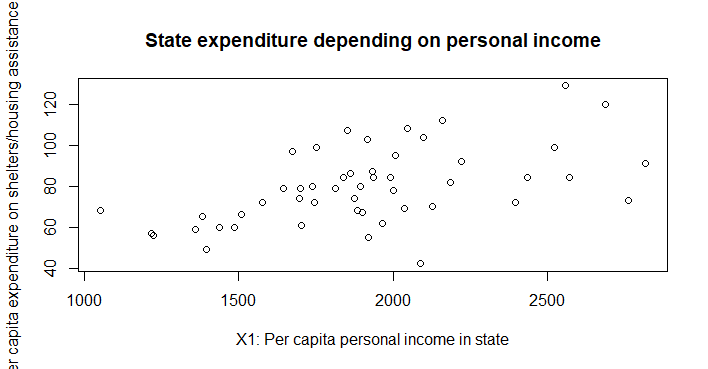
\includegraphics[width=.99\linewidth,height=.25\textheight,keepaspectratio]{Plot X1_Y}

\vspace{.25cm}
2) In the following plot of X2 and Y, it looks like there is no linear association between the variables. \\
\lstinputlisting[language=R, firstline=166, lastline=169]{PS01_answers_codefile_NF.R}
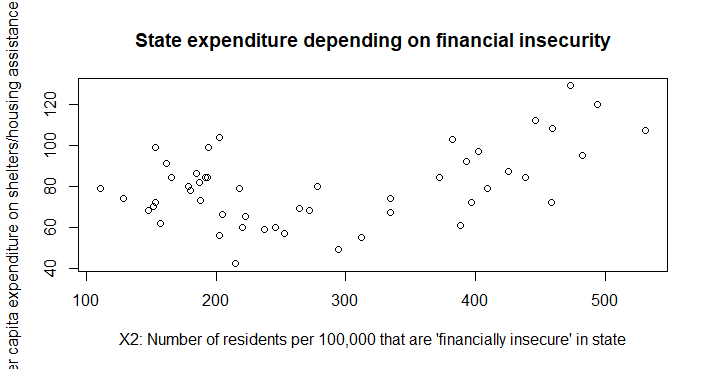
\includegraphics[width=.99\linewidth,height=.25\textheight,keepaspectratio]{Plot X2_Y}

\vspace{.5cm}
3) In the following plot of X3 and Y, it looks like there might be a slight positive correlation between the variables: the more people live in urban areas in state, the more states incur expenditure on housing assistance.
\lstinputlisting[language=R, firstline=173, lastline=176]{PS01_answers_codefile_NF.R} 
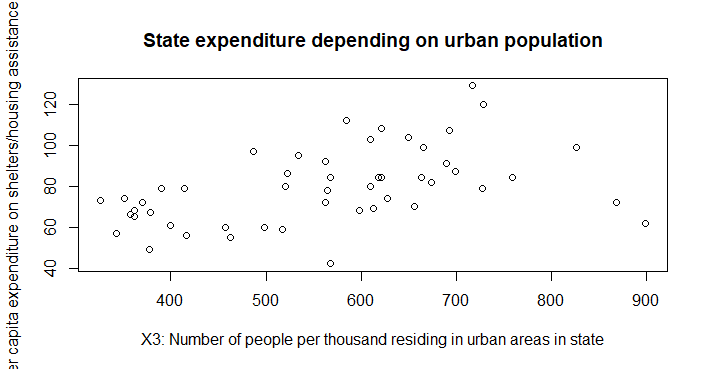
\includegraphics[width=.99\linewidth,height=.25\textheight,keepaspectratio]{Plot X3_Y}

\vspace{1cm}
4) In the following plot of X1 and X2, it looks like there is no linear association between both variables.
\lstinputlisting[language=R, firstline=181, lastline=184]{PS01_answers_codefile_NF.R} 
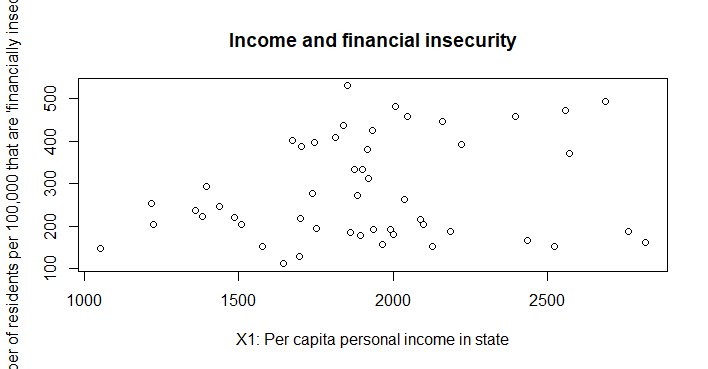
\includegraphics[width=.99\linewidth,height=.25\textheight,keepaspectratio]{Plot X1_X2}

\vspace{.5cm}
5) In the following plot of X1 and X3, it looks like there is no linear association between both variables.
\lstinputlisting[language=R, firstline=187, lastline=190]{PS01_answers_codefile_NF.R} 
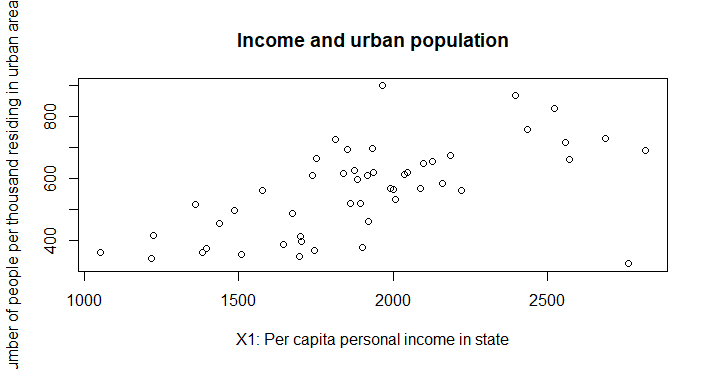
\includegraphics[width=.99\linewidth,height=.25\textheight,keepaspectratio]{Plot X1_X3}

\vspace{.25cm}
6) In the following plot of X2 and X3, it looks like there is no linear association between both variables.
\lstinputlisting[language=R, firstline=192, lastline=195]{PS01_answers_codefile_NF.R} 
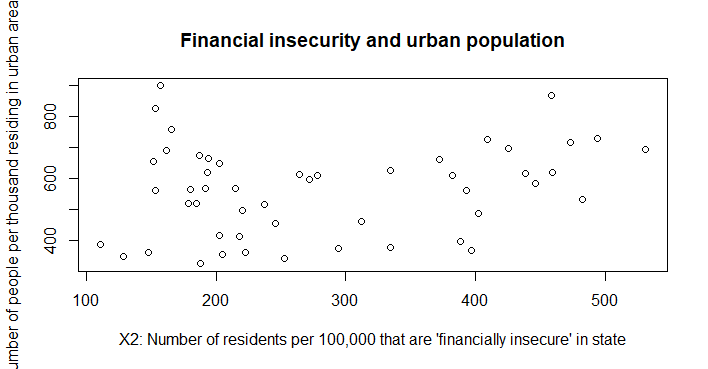
\includegraphics[width=.99\linewidth,height=.25\textheight,keepaspectratio]{Plot X2_X3}


\vspace{.5cm}
\item
Please plot the relationship between \emph{Y} and \emph{Region}? On average, which region has the highest per capita expenditure on housing assistance?
\vspace{.5cm}

Here is the plot representing the relationship between Y and Region:
\lstinputlisting[language=R, firstline=201, lastline=204]{PS01_answers_codefile_NF.R} 
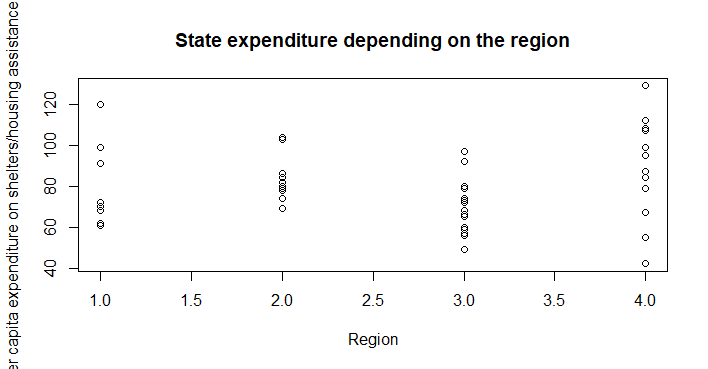
\includegraphics[width=.99\linewidth,height=.25\textheight,keepaspectratio]{Plot Y_region} \\
We can now calculate the means for each region and compare them:
\lstinputlisting[language=R, firstline=206, lastline=211]{PS01_answers_codefile_NF.R} 
Result: 
\begin{verbatim}
	table(region_mean$Region, region_mean$region_mean)
	
	69.1875 79.4444444444444 83.9166666666667 88.3076923076923
	1       0                9                0                0
	2       0                0               12                0
	3      16                0                0                0
	4       0                0                0               13
\end{verbatim}
We can conclude that the Western region has the highest per capita state expenditure on housing assistance.

\vspace{1cm}

\item
Please plot the relationship between \emph{Y} and \emph{X1}? Describe this graph and the relationship. Reproduce the above graph including one more variable \emph{Region} and display different regions with different types of symbols and colors. \\

Here is the plot showing the relationship between X1 and Y.
\lstinputlisting[language=R, firstline=158, lastline=161]{PS01_answers_codefile_NF.R} 
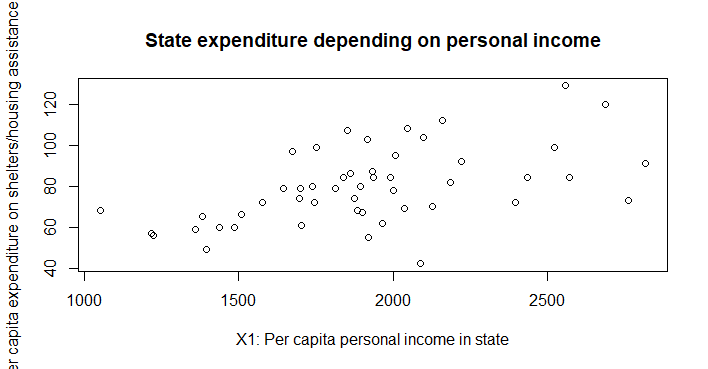
\includegraphics[width=.99\linewidth,height=.25\textheight,keepaspectratio]{Plot X1_Y} \\
As highlighted above, it looks like there is a positive correlation between X1 and Y: the higher the personal income of residents is, the more state incur expenditure on housing assistance. \\

Let's switch to ggplot to show this relationship with the added variable "Region":
\lstinputlisting[language=R, firstline=226, lastline=232]{PS01_answers_codefile_NF.R} 

\includegraphics[width=.99\linewidth,height=.99\textheight,keepaspectratio]{{Plot X1_Y_region}} \\

\end{itemize}


\end{document}
